\chapter{Embedding Methods: Preliminaries}
In this chapter we outline briefly terms and distinctions to be used by the embedding algorithms discussed in later chapters.

\section{Types and Tokens}
To process language, it is useful to make the following distinction between two ways of talking about at word-instances, identified by the different ways they are counted:
\begin{definition}[Types and tokens]
  When we count the number of unique vocabulary items in a document we call the things counted \emph{word-types}, whereas when we add up the number of words in a ``word count'' repetitions are permitted and we call the things counted \emph{word tokens}.
\end{definition}
Consider the following example:
\begin{example}[Types and tokens]\par
\phantom{line}
\authorquote{The limits of my language means the limits of my world}{\textcite{wittgenstein-1922-tract}}
This sentence contains $11$ word-tokens, but only $7$ word-types because the four words ``\emph{the limits of my}'' are each repeated once.
\end{example}
This distinction is very useful when processing language, however, as \textcite{kaplan-1990-words} notes, this type/token distinction is very much an \emph{orthographic} construction -this is most straightforwardly apparent in the case of identical tokens which represent separate ``grammatical words'' (like the different grammatical words `rock (music)' and `rock (stone)' both represented by the same orthographic word `rock' in \autoref{fig:polysemy}). \citeauthor{kaplan-1990-words} discusses the shortcomings of this type/token model as a tool for \emph{understanding} language in depth, asserting ``The criterion of word identity is not resemblance'' -however, whether this distinction has \emph{explanatory power} regarding language or otherwise, it inarguably has \emph{utility} when processing language.

\section{Distributional Similarity \& Semantic relatedness}\label{sec:semantic-relatedness}
Up until this point we have used the terms ``semantic relatedness'' and ``word similarity'' interchangeably without clarifying what we are referring to in either case. We have said that word embedding algorithms use observed \emph{distributional similarity} to infer underlying \emph{semantic relatedness/word similarity}, but not discussed the specifics of this inference. In this section we first define a variety of ways in which words can be semantically related, then we discuss types of distributional similarity which can reveal semantic relations, and finally we discuss the limits of this methodology.

We reference \citeauthor{turney10-from-frequen-to-meanin}'s \parencite*{turney10-from-frequen-to-meanin} framework for distinguishing between types of semantic relatedness. First, they describe the general concept of semantic relatedness as follows:

\basicquote{The term semantic relatedness in computational linguistics \parencite{budanitsky-2001-semantic-distance} corresponds to attributional similarity in cognitive science \parencite{gentner-1983-structure-mapping}. Two words are semantically related if they have any kind of semantic relation \parencite{budanitsky-2001-semantic-distance}; they are semantically related to the degree that they share attributes \parencite{turney-2006-similarity}. Examples are synonyms (bank and trust company), meronyms (car and wheel), antonyms (hot and cold), and words that are functionally related or frequently associated (pencil and paper). We might not usually think that antonyms are similar, but antonyms have a high degree of attributional similarity (hot and cold are kinds of temperature, black and white are kinds of colour, loud and quiet are kinds of sound).}

Then they present two particular semantic relations (``taxonomic similarity'' and ``semantic association'') which can be characteristically linked with distributional circumstances (termed ``paradigmatic parallels'', or ``syntagmatic associates'' \textcite{shutze-1993-word-space}). We paraphrase their definitions here:
\begin{infobox}{Types of semantic relation  \parencite{turney10-from-frequen-to-meanin}, \& related manners of distribution \parencite{resnik-1995-nov}}
  The following ways that words can be semantically related: 
    \paragraph{Semantic association} Words which tend to co-occur frequently (e.g. \emph{bee} and \emph{honey})
    \paragraph{Taxonomic similarity} Words which share a hypernym (\emph{car} and \emph{bicycle} are taxonomically similar, because they share the hypernym \emph{vehicle}).

    \noindent
    Are associated with these two following manners in which words can be \emph{distributionally} related:
    \paragraph{Syntagmatic associates} Words which tend to be each other's neighbours.
      \paragraph{Paradigmatic parallels} Words which tend to share the same neighbours.
\end{infobox}
This link between semantic relation and distributional is justified by the observation that words which are each other's neighbours (syntagmatic associates like \emph{bee} and \emph{honey}) ``are often different parts of speech'', whereas words which share similar neighbours (taxonomically similar words like \emph{doctor} and \emph{nurse}) ``are usually the same part of speech''.

The inference we can make based on distributional conditions then, is this:
\begin{align}
  \text{\fbox{\emph{syntagmatic associates}}}&\implies\text{\fbox{\emph{\vphantom{g}semantic associates}}}\\
  \text{\fbox{\emph{paradigmatic parallels}}}&\implies\text{\fbox{\emph{taxonomically similar}}}
\end{align}
\noindent
We will discuss in the following chapters how co-occurrence matrix based embedding methods algorithms can be used to generate word spaces reflecting more \emph{syntagmatic association} or \emph{paradigmatic parallel} type distributional relationships. As you will see, however, the ability to target specific semantic relationships with these algorithms is quite coarse-grained -even if these two categories of semantic relation (semantic association and paradigmatic parallelism) could be captured with some precision, what about the more specific types of relation mentioned by \citeauthor{turney10-from-frequen-to-meanin} (synonymy, meronymy \& antonymy) at the start of this section, or other relations?

\authorquote{A commonly raised criticism for both types of semantic space models (i.e., word-based and syntax-based)\footnotemark  concerns the notion of semantic similarity. Proximity between two words in the semantic space cannot indicate the nature of the lexical relations between them. Distributionally similar words can be antonyms, synonyms, hyponyms or in some cases semantically unrelated. This limits the application of semantic space models for NLP tasks which require distinguishing between lexical relations}{\textcite{pado-lapata-2003-constructing}}
\footnotetext{The term ``syntax based'' used in contrast to ``word based'' refers to models which make use of an a-priori encoded conception of word-order relationships like {\small SUBJECT-OBJECT}.}
\noindent
This limit of word space models (referred to as \emph{semantic space models} by \citeauthor{pado-lapata-2003-constructing} above) is in fact essential to their construction. The semantic relatedness they model is of a more general nature. This is not necessarily a shortcoming of the models however. \textcite{sahlgreen-2006-the-word-space-model} writes in his thesis:
\basicquote{This criticism is arguably valid from a prescriptive perspective where these relations are a priorily given as part of the linguistic ontology. From a descriptive perspective, however, these relations are not axiomatic, and the broad notion of semantic similarity seems perfectly plausible. There are studies that demonstrate the psychological reality of the concept of semantic similarity. For example, \textcite{miller-1991-contextual-correlates} [\dots]; people appear to instinctively understand what semantic similarity is [\dots]. Several researchers report high inter-subject agreement when asking a number of test subjects to provide semantic similarity ratings for a given number of word pairs \parencite{rubenstein-1965-contextual-correlates, henley-1969-a-psychological, miller-1991-contextual-correlates}}
Indeed, it is not clear how these more particular semantic relationships \emph{could} be captured by the arrangements of points in a word space -\citeauthor{sahlgreen-2006-the-word-space-model} continues:
\basicquote{the nature of the similarities in the word-space model is a consequence of using the distributional methodology as discovery procedure, and the geometric metaphor of meaning as representational basis. [...] If we want to claim that we extract and represent some particular type of semantic relation in the word-space model, we need to modify either the distributional hypothesis or the geometric metaphor.}

\section{Pointwise Mutual information}
%% The first is the most well known statement of \emph{quantitative linguistics}: an empirical observation about statistical regularities of written language known as \emph{Zipf's Law}.
%% 
%% \begin{definition}[Zipf's Law]\label{def:zipf}
  %% In 1932 George Zipf published an observation about the relationship between \emph{the rank of a word in a vocabulary list ordered from most frequent to least frequent}, and \emph{the frequency of that word} (in a particular body of text).\par\noindent
  %% Let the rank of a word in a vocabulary list ordered from most-to-least frequent be $r$, and $f(r)$ be the normalised frequency count for that word (i.e., the number of times that word appears in the text divided by the total number of words $N$). Then Zipf's law states the following equality will hold approximately:
  %% \begin{equation}
    %% f(s)=\frac{A}{s^\alpha}
  %% \end{equation}
  %% where $A$ is a normalising constant, and $\alpha$ is a value slightly greater than $1$.
%% \end{definition}
%% Zipf first stated this observation slightly differently, he noted that the product of the absolute frequencies (we write $f^*(r)$, -note $f(r)=f^*(r)/N$) and the rank $r$ approximated a constant:
%% \begin{equation}
  %% r\times f^*(r)= C \label{eq:zipf-rectangular}
%% \end{equation}
%% In his original exposition, Zipf provides the following table (abbreviated here) tallying frequencies of words in James Joyce's \emph{Ulysses} as motivation for the statement of \eqref{eq:zipf-rectangular}:\par\vspace{1em}
%% \begin{center}
  %% \captionsetup{width=.91\linewidth}
  %% \begin{tabular}{r r r}
    %% \toprule
    %% I: Rank ($r$) & II: Frequency ($f^*(r)$) & III: The product of I \& II \\
    %% \midrule
    %% 10     &  2,653 & 26,530 \\
    %% 20     &  1,311 & 26,220 \\
    %% 30     &    926 & 27,780 \\
    %% 40     &    717 & 28,680 \\
    %% 50     &    556 & 27,800 \\
    %% \vdots & \vdots & \vdots \\
    %% 1,000  &     26 & 26,000 \\
    %% 2,000  &     12 & 24,000 \\
    %% 3,000  &      8 & 24,000 \\
    %% 4,000  &      6 & 24,000 \\
    %% 5,000  &      5 & 25,000 \\
    %% \vdots & \vdots & \vdots \\
    %% \bottomrule
  %% \end{tabular}
  %% \captionof{table}{Frequency counts for words from \emph{Ulysses} collated as evidence for the early formulation of ``Zipf's Law''.}
%% \end{center}
%% This form \eqref{eq:zipf-rectangular} can then be rearranged to yield the form referenced in \nameref{def:zipf} (without the exponent in the denominator):
%% \begin{align}
  %% f^*(r)&=\frac{C}{r}\\[6pt]
  %% f(r)&=\frac{A}{r}\raisebox{6pt}{\;(\;=C/N)}
%% \end{align}
%% The exponent $\alpha$, as can be observed in \autoref{fig:zipf-chart} is due to further empirical investigation revealing that the relationship deviates slightly from the original equation.
%% \begin{figure}[H]
  %% \centering
  %% \captionsetup{width=.91\linewidth}
  %% 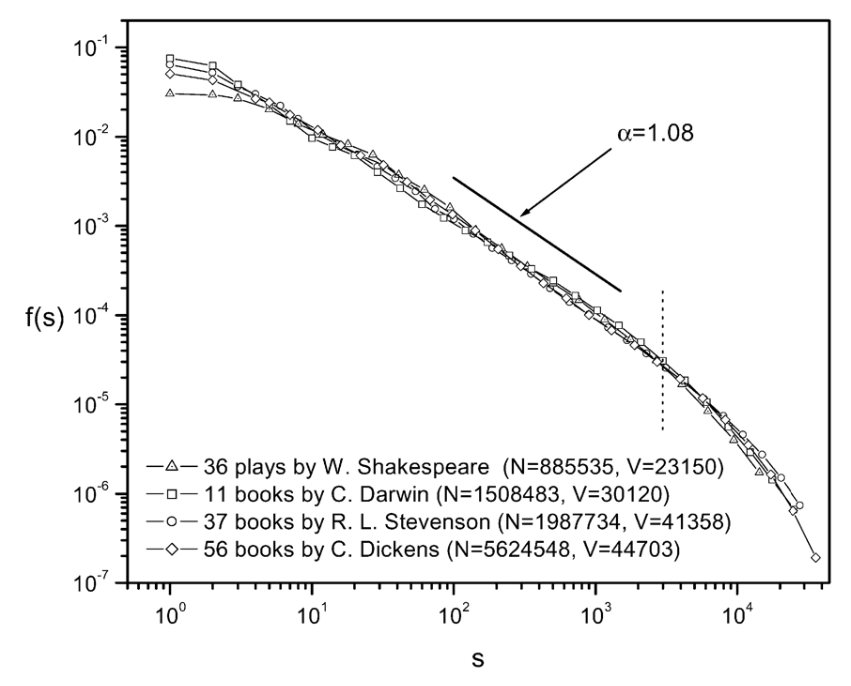
\includegraphics[scale=0.35]{figures/zipf-chart.png}
  %% \caption{Chart from \parencite{montemurro-2001-beyond-the-zipf} -``Frequency-rank distribution of words for four large text samples. In order to reveal individual variations these corpora are built with literary works of four different authors, respectively.  The vertical dash line is placed approximately where Zipf’s law ceases to hold''.}\label{fig:zipf-chart}
%% \end{figure}
%% As \textcite{montemurro-2001-beyond-the-zipf} note regarding the above figure, the relationship does not hold absolutely for lower frequency words. In their paper \parencite{montemurro-2001-beyond-the-zipf} they present a more detailed model capturing this variation. Their improved model is beyond the scope of this report but is illustrative of the difficulties of processing low-frequency words in particular, an issue we come across again later in this report.
%% 
The next concept is from the field of information theory and measures the amount of information revealed about a system when its outcome is partly decided. It is useful in embedding processes for quantifying how novel it is for two words to have co-occurred together (very frequent words like ``the'' are less novel partners to co-occur with than more domain-specific terms).

\begin{definition}[Pointwise Mutual Information]
  Given two discrete random variables with a joint distribution $P:X\times Y\to [0,1]$, such that the probability of $x$ and $y$ co-occurring is given by $P(x,y)$, the \emph{pointwise mutual information} of $x$ and $y$ is given by:
  \begin{equation}
    I(x,y)=\log\frac{P(x,y)}{P(x)P(y)}\label{eq:pmi}
  \end{equation}
\end{definition}

Pointwise mutual information is a measure of how much information about one random variable's value is gained, given that the value taken by the other is already known. For this reason it is natural to describe it in terms of conditional probabilities:
\begin{equation}
  I(x,y)=\log\frac{P(x\mid y)}{P(x)}
\end{equation}
This value happens to be symmetric with respect to $x$ and $y$:
\begin{equation}
  I(x,y)= \log\frac{P(x\mid y)P(y)}{P(x)P(Y)}\ =\ \log\frac{P(y\mid x)P(x)}{P(y)P(x)}=\log\frac{P(x, y)}{P(x)P(y)}
\end{equation}
which is why it is called the pointwise \emph{mutual} information.

If all outcomes in a joint distribution are equally likely, then learning the value of one of the variables does not give you any new information about the probability that the remaining variable takes any particular value. If the two are highly dependent on one another however, the outcome of one can be very informative about the probable outcomes for the other. This is the intuition which pointwise mutual information formalises.
\begin{example}[Pointwise mutual information] Given the definition we expect that for the two joint distributions ($P_1$, $P_2$, on $X$ and $Y$ shown in \autoref{tab:pmi1} and \autoref{tab:pmi2}), in the first case the pointwise mutual information for particular values (we choose $x_3$ and $y_3$) would be none, and in the second case would be positive. We calculate both below, referring to the first value $I_1$ and the second $I_2$.
  \phantom{para}\\\vspace{-3em}\par\hfill\allowbreak{}\\
  \hspace{-1.5em}
  \begin{minipage}{.5\textwidth}
  \vspace{0pt}
    \begin{center}\begin{tabular}{c R R !{\color{red}\vrule width 0.5pt} R !{\color{red}\vrule width 0.5pt} R r}
      \multicolumn{1}{c}   {  } & \multicolumn{1}{c} {$z_1$} & \multicolumn{1}{c} {$x_2$} & \multicolumn{1}{c} {$x_3$} & \multicolumn{1}{c} {$x_4$} & \multicolumn{1}{c} {}\\
      $y_1$ &  1/16  &  1/16  & 1/16 & 1/16    & \hspace{1em} 0.25\\
      $y_2$ &  1/16   &  1/16   & 1/16  & 1/16 & \hspace{1em} 0.25\\\hhline{~>{\arrayrulecolor{red}}----~}
      $y_3$ &  1/16  &  1/16  & 1/16 & 1/16    & \hspace{1em} 0.25\\\hhline{~>{\arrayrulecolor{red}}----~}
      $y_4$ &  1/16  &  1/16   & 1/16  & 1/16  & \hspace{1em} 0.25\\[0em]\\[-1em]
      \multicolumn{1}{c}   {} & \multicolumn{1}{c} {0.25} & \multicolumn{1}{c} {0.25} & \multicolumn{1}{c} {0.25} & \multicolumn{1}{c} {0.25} & \multicolumn{1}{c} {1}\\
    \end{tabular}\end{center}
  \captionof{table}{Case 1: $X$ and $Y$ with constant joint distribution $P_1$.}\label{tab:pmi1}
\end{minipage}
\hspace{1.4em}
\begin{minipage}{.5\textwidth}
  \vspace{0pt}
    \begin{center}\begin{tabular}{c R R !{\color{red}\vrule width 0.5pt} R !{\color{red}\vrule width 0.5pt} R r}
      \multicolumn{1}{c}   {  } & \multicolumn{1}{c} {$x_1$} & \multicolumn{1}{c} {$x_2$} & \multicolumn{1}{c} {$x_3$} & \multicolumn{1}{c} {$x_4$} & \multicolumn{1}{c} {}\\
      $y_1$ &  0.08  &  0.09  & 0.03 & 0.06    & \hspace{1em}0.26\\
      $y_2$ &  0.05   &  0.08   &  0.04 & 0.13 & \hspace{1em}0.30 \\\hhline{~>{\arrayrulecolor{red}}----~}
      $y_3$ &  0.11  &  0.03  & 0.03 & 0.06    & \hspace{1em}0.23 \\\hhline{~>{\arrayrulecolor{red}}----~}
      $y_4$ &  0.05  &  0.10   &  0.02 & 0.04  & \hspace{1em}0.21\\[0em]\\[-1em]
      \multicolumn{1}{c}   {} & \multicolumn{1}{c} {0.29} & \multicolumn{1}{c} {0.30} & \multicolumn{1}{c} {0.12} & \multicolumn{1}{c} {0.29} & \multicolumn{1}{c} {1}\\
    \end{tabular}\end{center}
  \captionof{table}{Case 2: $X$ and $Y$ with varied joint distribution $P_2$.}\label{tab:pmi2}
  \end{minipage}
  \phantom{para}\\[0.8em]
  \begin{align*}
    I_1(x_3,y_3)=\log\frac{P_1(x_3,y_3)}{P_1(x_3)P_1(y_3)}&=\log\frac{1/16}{0.25\cdot 0.25}\\
                                                          &=\log 1\ (= 0)\tag{first case}\\[1.5em]
    I_1(x_3,y_3)=\log\frac{P_2(x_3,y_3)}{P_2(x_3)P_2(y_3)}&=\log\frac{0.03}{0.23\cdot 0.12}\\
                                                          &=\log \frac{25}{23}\ (> 0)\tag{second case}
  \end{align*}
  You can see that the calculated PMI values conform with the intuition we described above.
  \vspace{0.0em}
\end{example}

\section{Tokenizing}
In this section we present a formal description of \emph{tokens}, the core unit upon which embedding algorithms operate on, in mathematical language. We did not find a formal description of tokens as mathematical elements like this in the literature -it is often assumed that a tokenized corpus is already prepared and understood- so we briefly present our own.

Since one of our aims in this report is to highlight the fact that many key ideas used to generate word spaces do not \emph{assume} that the objects being operated on are actually words (discussed in \nameref{chap:beyond-word-embeddings}), we thought a formal description of type of input generally expected by these algorithms would be a useful detail to specify.
\begin{definition}[Orthography]\label{def:orthography}
  An orthography is a finite set of symbols.
\end{definition}

\begin{example}\label{ex:orthographies}
  The sets:
  \begin{align}
    &\mathscr{O}_P=\{\mycirc[green], \mycirc[blue], \mycirc[red]\}\label{eq:dots-orthography}\\
    &\mathscr{O}_L=\{c\mid\text{$c$ is a letter, number or special character marked on \autoref{fig:uk-keyboard}}\}\label{eq:keyboard-orthography}
  \end{align}
  are both examples of orthographies.
\end{example}
\vspace{6pt}

\begin{figure}[ht]
 \centering
 \includesvg[width=0.9 \columnwidth]{figures/inkscape/uk-keyboard.svg}
 \caption{A standard uk keyboard layout}
 \label{fig:uk-keyboard}
\end{figure}

\begin{definition}[Document]
  A document $d$ is a finite sequence $c_0,c_1,\dots,c_n$ ($c\in\mathscr{O}$), where $\mathscr{O}$ is an orthography.
\end{definition}

\begin{example}[Dots Documents]\label{ex:doc-plato}
  The sequence of symbols:
  \[
    d_1=\fbox{\mycirc[red] \mycirc[green] \mycirc[blue] \mycirc[blue] \mycirc[red] \mycirc[blue] \mycirc[red] \mycirc[green] \mycirc[blue] \mycirc[green]}\label{eq:dots-document}
  \]
  is a document using orthography \eqref{eq:dots-orthography}.
\end{example}

\begin{example}[Plato Documents]\label{ex:doc-plato}
    Plain text versions of the complete works of Plato (English translations) are available at the \href{https://www.gutenberg.org/ebooks/author/93}{Project Gutenberg} website. These are examples of documents using keyboard orthography \ref{eq:keyboard-orthography} referenced above.
\end{example}

\begin{definition}[Word-Token]
  A word token $w$ is like a document -it is a sequence of symbols $c_0,c_1,\dots,c_n$ ($c\in\mathscr{O}$ from an orthography $\mathscr{O}$. The difference between a word token and a document is context: we call a sequence of symbols from an orthography a \emph{word token} when it is the output of a tokenizer (defined next).
\end{definition}

\begin{definition}[Tokenizer]
   A tokenizer $T$ is a function that maps a document to a sequence of word tokens; $T(d)=w_1,w_2,\dots,w_n$. The output is referred to as the 'tokenized' form of the document. We use the shorthand $W_d$ to refer to the tokenized document $T(d)$ when it is clear which tokenization has been used.\footnotemark.
\end{definition}
\footnotetext{Here we consider tokenization in an abstract sense essentially saying ``A tokenizer is a function that extracts tokens''. For a practical look at pre-processing see \nameref{chap:further-reading}.}

\begin{example}[Dots Document Tokenized]\label{ex:doc-plato}
  Using the tokenizing procedure: \emph{treat blue dots as token-deliminators}, the tokenization of document \eqref{eq:dots-document} yields:
  \begin{align}
    T(d_1)&=\fbox{\mycirc[red] \mycirc[green]}, \fbox{\mycirc[red]}, \fbox{\mycirc[red] \mycirc[green]}, \fbox{\mycirc[green]}\label{eq:dots-tokenized}\\
    &=W_{d_1}\nonumber
  \end{align}
\end{example}

\begin{example}[Simple Text Tokenizer]\label{ex:simple-tokenizer}
  In \autoref{alg:simple-tokenizer} we present a simple algorithm for tokenizing text which ignores a predefined list of special symbols, and identifies token-boundaries using predefined deliminator symbols.

  Setting {\sffamily ignore}$=("!", ".", ",", ";", ":", "'")$, and {\sffamily deliminators}$=("~")$, the following document:
  \begin{equation*}
    d_2=\text{\fbox{Predicting is difficult -especially about the future.}}
  \end{equation*}
  using the orthography \eqref{eq:keyboard-orthography} has the tokenized form:
  \begin{align}
    T(d_2)&=\text{\fbox{Predicting}}, \text{\fbox{is\vphantom{gt}}}, \text{\fbox{difficult\vphantom{gt}}}, \text{\fbox{-especially\vphantom{gt}}}, \text{\fbox{about\vphantom{gt}}}, \text{\fbox{the\vphantom{gt}}}, \text{\fbox{future\vphantom{gt}}}\label{eq:sentence-tokens}\\
    &=W_{d_2}\nonumber
  \end{align}
  Clearly the token \fbox{-especially} is not in the form an English speaker would transcribe if tasked with tokenizing the sentence by hand -but we use this example to highlight the difficulty of tokenizing: with this approach hyphenated expressions like ``brother-in-law'' will be correctly tokenized as single units, but in cases like \eqref{eq:sentence-tokens} mistakes are made. It is not possible to handle both cases correctly with our simple algorithm.
\end{example}

\begin{figure}[H]
  \centering
  \captionsetup{width=.91\linewidth}
  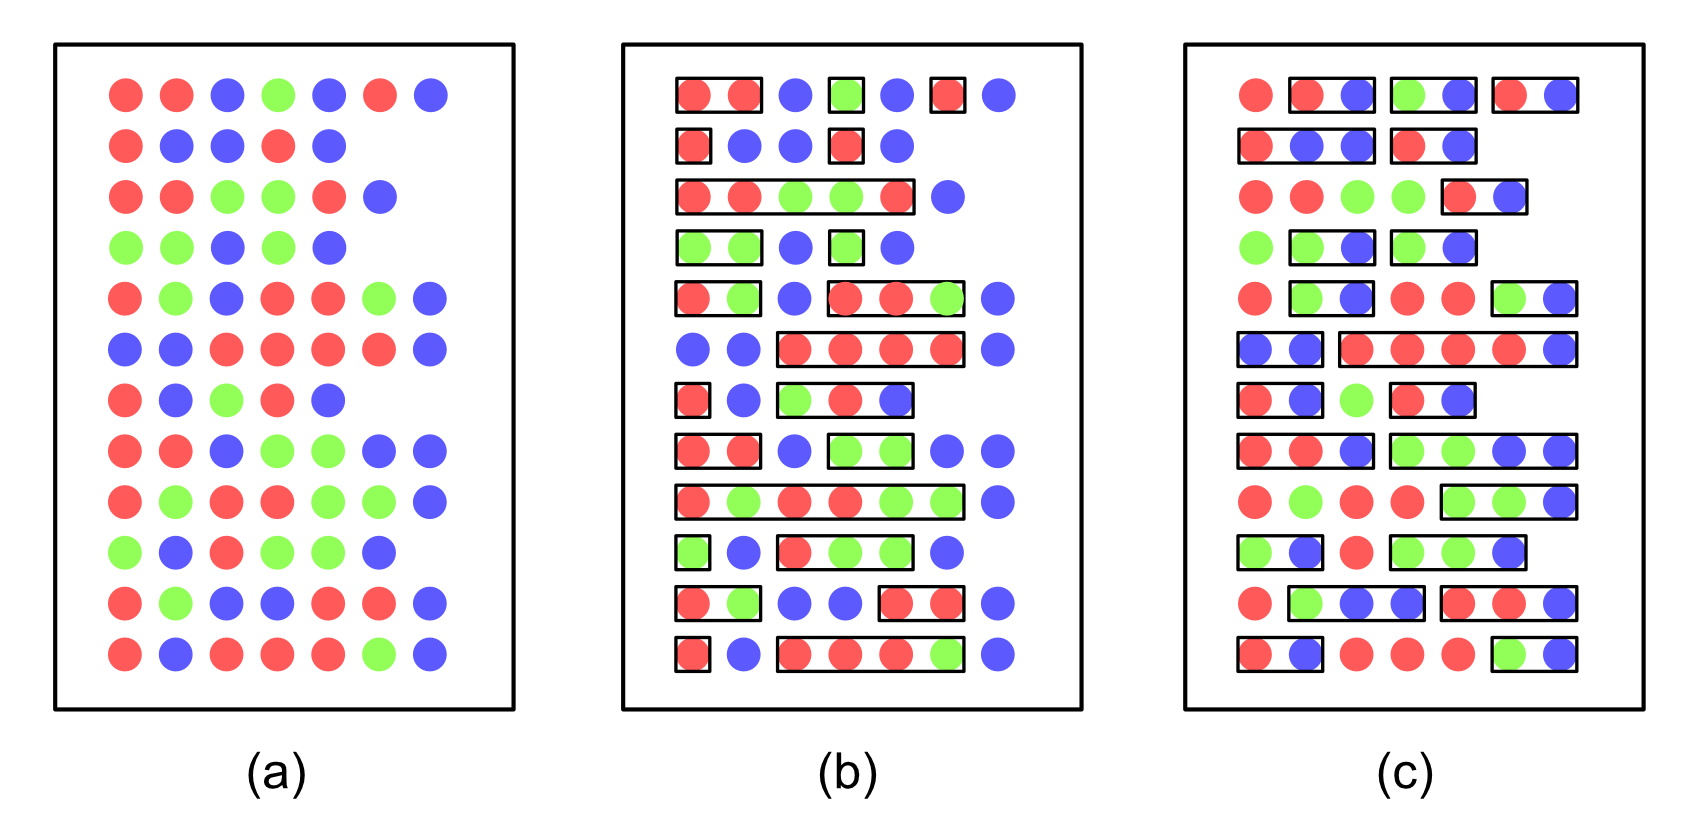
\includegraphics[scale=0.70]{figures/affinity-designer/tokens.png}
  \caption{Tokens identified by two different tokenizations, (b) \& (c), performed on the same document (a) (using the orthography~\eqref{eq:dots-orthography}). The tokenizer used in the case of (b) identifies tokens as sequences of red and green dots delimited by blue dots, and for (c) the tokenizer identified tokens as sequences of consecutive repeated symbols which are terminated by any number of blue dots.}\label{fig:dot-tokenizers}
\end{figure}
\par
\begin{algorithm}
  {\small
  \caption{Simple Text Tokenizer}\label{alg:simple-tokenizer}
  \SetNoFillComment{}
  \DontPrintSemicolon{}
  \SetKwData{Tokens}{tokens}
  \SetKwData{NextToken}{next\_token}
  \SetKwData{Ignore}{ignore}
  \SetKwData{Delim}{deliminators}
  \SetKwData{Doc}{document}
  \SetKwData{Symb}{symbol}
  \SetKwFunction{Append}{append}
  \SetKwFunction{List}{list}
  \SetKwFunction{Return}{return}
  \SetKwFunction{Preprocess}{preprocess}
  \SetKwInOut{Input}{input}\SetKwInOut{Output}{output}

  \Input{A list of symbols: \Doc, a list of ignored ``special'' symbols: \Ignore, and a list of deliminator symbols: \Delim}
  \Output{A list of word tokens: \Tokens}
  \BlankLine

  \Tokens $\leftarrow$ \List{}\;
  \NextToken $\leftarrow$ \List{}\;
  \tcc{Go through the document one symbol at a time, skipping special characters, and adding \NextToken to \Tokens when a deliminator is reached}
  \For{\Symb in \Doc}{
    \uIf{\Symb is in \Delim}{
      \tcc{Add \NextToken to \Tokens if \NextToken only if it contains symbols}
      \uIf{\NextToken is not empty}{
        \Tokens$\leftarrow$ \Append{\NextToken, \Tokens}\;
        \NextToken$\leftarrow$ \List{}\;
      }
      \Else{
        \tcc{Keep parsing symbols to add to \NextToken until the next deliminator is reached}
      }
    }
    \uElseIf{\Symb is in \Ignore}{
      \tcc{Ignore this symbol}
    }
    \Else{
      \tcc{Add this symbol to the \NextToken variable}
      \NextToken$\leftarrow$ \Append{\Symb, \NextToken}\;
    }
  }
  \Return{\Tokens}
  }
\end{algorithm}
\par
We have described tokenization for orthographies of letter-based and dot-based documents but of course there are many other possibilities, for example tokenizing musical notation by delimiting tokens at bar-boundaries.

\begin{definition}[Corpus]
  A corpus $C$ is a finite set of documents $\{d_1, d_2,\dots,d_n\}$, $n\in\mathbb{N}$.
\end{definition}

\begin{example}[Plato Corpus]\label{ex:corp-plato}
  The complete works of Plato in plain-text form, referenced in \autoref{ex:doc-plato} is an example of a corpus.
\end{example}

\begin{definition}[Vocabulary]
  The vocabulary of a tokenized document $W_d$ is the set of unique word tokens in the tokenization of that document; $V(W_d)=\{w\mid w\in\, \text{the sequence $W_d$}\}$. The vocabulary of a corpus is the union of the vocabularies of each document in that corpus; $V(C)=V(W_{d_1})\cup V(W_{d_2})\cup \dots\cup V(W_{d_n})$.
\end{definition}

\begin{definition}[$\#$ Operator]
  The $\#$ symbol, used preceding a set or a sequence, denotes ``the number of elements in''. $\#W_d$ denotes the number of tokens in the tokenized form of document $d$ then, and $\#V(W_d)$ denotes the vocabulary size of document $d$.
\end{definition}

\begin{example}[Dots Document Properties]
  The vocabulary of the tokenized document \eqref{eq:dots-tokenized} is:
  \begin{align*}
    V(W_{d_1})&=V(\fbox{\mycirc[red] \mycirc[green]}, \fbox{\mycirc[red]}, \fbox{\mycirc[red] \mycirc[green]}, \fbox{\mycirc[green]})\\
              &=\{\fbox{\mycirc[red] \mycirc[green]}, \fbox{\mycirc[red]}, \fbox{\mycirc[green]}\}
  \end{align*}
  The number of tokens (the word count) for this document is: $\#W_{d_1}=4$ and the vocabulary size is $\#V(W_{d_1})=3$
\end{example}

\begin{example}[Plato Document Sizes]
  Word token counts and vocabulary sizes for a selection Plato documents from~\ref{ex:doc-plato}, tokenized using a variation of the simple tokenizer\footnotemark described by \autoref{alg:simple-tokenizer}, are listed here:\\[-1em]
  \begin{center}
  \captionsetup{width=.91\linewidth}
    \begin{tabular}{c r r r r r r}
      \toprule
      \multicolumn{1}{c}{Attribute$\quad$} &
      \multicolumn{6}{c}{Document ($d$)} \\

      \cmidrule(lr){2-7}
      &
      $\texttt{laws}$ &
      $\texttt{republic}$ &
      $\texttt{cratylus}$ &
      $\texttt{meno}$ &
      $\texttt{apology}$ &
      $\texttt{crito}$ \\
      \midrule
      $\#W_d$ & 140,406 & 118,283 & 23,883 & 12,716 & 11,392 & 5,332\\
      $\#V(W_d)$ & 8,100 & 8,105 & 2,963 & 1,493 & 1,789 & 1,030\\
      \bottomrule
    \end{tabular}
    \captionof{table}{Number of Word Tokens \& Vocabulary Sizes of a selection of Documents in the Plato Corpus (\autoref{ex:corp-plato})}
    \end{center}
\end{example}
\footnotetext{The code used to produce this table, and other examples using this data set, is available on \href{https://github.com/joelstrouts/degree-project}{Github}.}

\begin{example}[Plato Corpus Size]
  The complete Plato corpus (\ref{ex:corp-plato}) consists of 25 documents and, each tokenized the same way as before, has the word count $\sum_{d\in C_P}\#W_d=670,936$ and the vocabulary size $\#V(C_P)=19,432$.
\end{example}
\noindent
These are the essential mathematical objects which are used to construct co-occurrence matrices as we describe in the following chapter.

\section{Similarity Measure}
There are many possible measures of similarity for comparing two vectors, but in the word embedding domain by far the most prevalent is the cosine similarity. We present only this method, but suggest reading \textcite{bullinaria-2007-extracting-semantic} for a discussion and comparison of other distance measuring approaches.

\begin{definition}[Cosine Similarity]
  Give two non-zero vectors $\bf{x}$ and $\bf{y}$, the cosine similarity between these two vectors is given by:
  \begin{equation}
    \operatorname{sim}(\bf{x}, \bf{y})=\frac{\bf{x}\cdot\bf{y}}{||\bf{x}||||\bf{y}||}
  \end{equation}
  where $\bf{x}\cdot\bf{y}$ is the dot product of $\bf{x}$ and $\bf{y}$ and $||\bf{v}||$ is the norm of $\bf{x}$.
  This formula is derived from the dot product formula: $\bf{x}\cdot\bf{y}=||\bf{x}||||\bf{y}||\cos\theta$.
\end{definition}

%%% Local Variables:
%%% mode: latex
%%% TeX-master: "../main"
%%% End:
